\documentclass[fleqn,10pt]{wlscirep}
\usepackage[utf8]{inputenc}
\usepackage[T1]{fontenc}
\usepackage{graphicx,verbatim}
\usepackage{array} % preamble에 이미 있을 수 있음
\usepackage{url}
\usepackage{cite}
\usepackage{amsmath,amssymb,amsfonts}
\usepackage{algorithmic}
\usepackage{graphicx}
\usepackage{textcomp}
\usepackage{xcolor}
\usepackage{multirow}
\usepackage{booktabs}  % \toprule, \midrule, \bottomrule
\usepackage{colortbl}
\usepackage{kotex}
\usepackage{soul}
\usepackage{subcaption}
\usepackage{pifont}
\usepackage{adjustbox}
\usepackage{threeparttable}
\usepackage{tikz}
\usepackage{pgfplots}
\pgfplotsset{compat=1.18}
\usetikzlibrary{positioning}
\newcommand{\cmark}{\ding{51}} % 체크 ✓
\newcommand{\xmark}{\texttimes} % × 기호 (얇음, 보통 수학 모드에서 많이 씀)
\bibliographystyle{unsrt}

\usepackage{booktabs}
%\usepackage{tabularx}


\newtheorem{theorem}{Theorem}
\newtheorem{defn}{Definition}
\newtheorem{remark}{Remark}
\newtheorem{assumption}{Assumption}

\begin{document}


\renewcommand{\arraystretch}{1.2}



\begin{figure}[htbp]
\centering
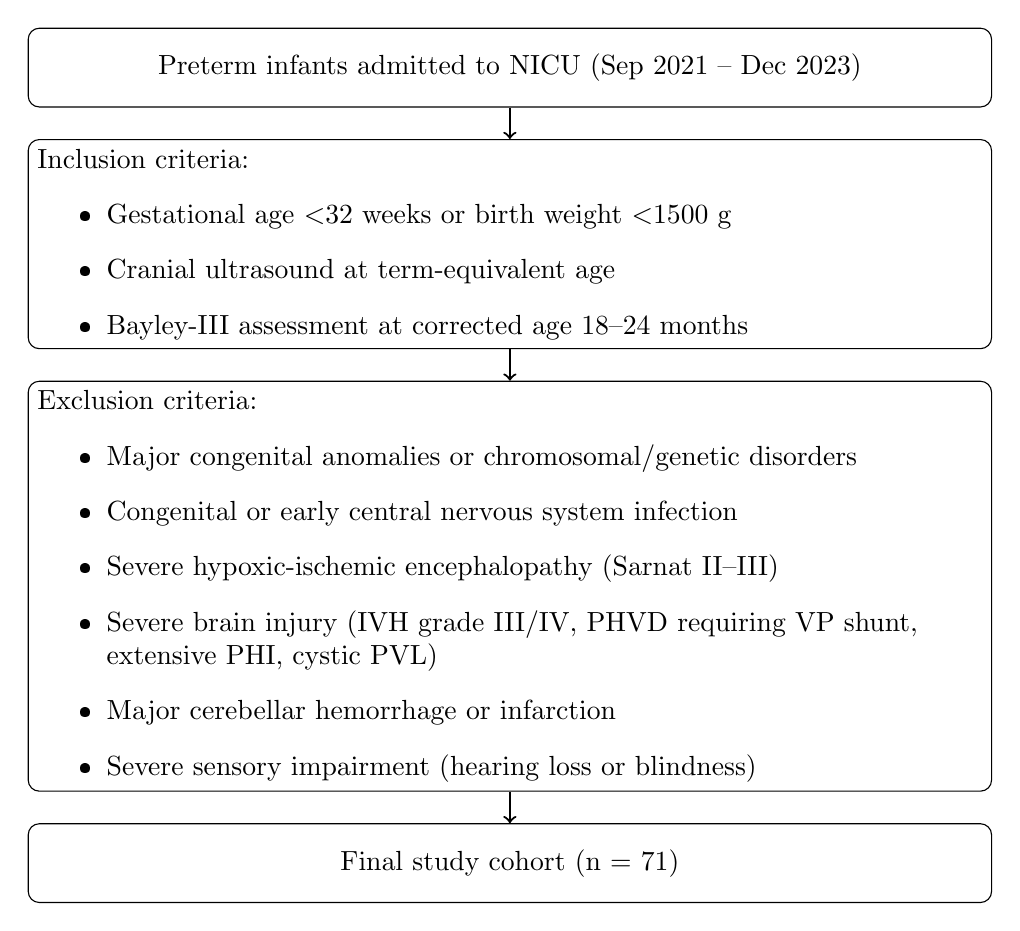
\begin{tikzpicture}[
    box/.style={rectangle, draw, rounded corners, text width=12cm, align=left, minimum height=1cm},
    arrow/.style={->, thick}
]

\node[box, align=center] (a) {Preterm infants admitted to NICU (Sep 2021 -- Dec 2023)};

\node[box, below=0.4cm of a] (b) {Inclusion criteria:
\begin{itemize}
\item Gestational age $<$32 weeks or birth weight $<$1500 g
\item Cranial ultrasound at term-equivalent age
\item Bayley-III assessment at corrected age 18--24 months
\end{itemize}
};

\node[box, below=0.4cm of b] (c) {Exclusion criteria:
\begin{itemize}
\item Major congenital anomalies or chromosomal/genetic disorders
\item Congenital or early central nervous system infection
\item Severe hypoxic-ischemic encephalopathy (Sarnat II--III)
\item Severe brain injury (IVH grade III/IV, PHVD requiring VP shunt, extensive PHI, cystic PVL)
\item Major cerebellar hemorrhage or infarction
\item Severe sensory impairment (hearing loss or blindness)
\end{itemize}
};

\node[box, below=0.4cm of c, align=center] (d) {Final study cohort (n = 71)};

\draw[arrow] (a) -- (b);
\draw[arrow] (b) -- (c);
\draw[arrow] (c) -- (d);

\end{tikzpicture}
\caption{Flow diagram of study population selection}
\label{fig:flow}
\end{figure}



\begin{table}[htbp]
\centering
\caption{Clinical, cranial ultrasound, and neurodevelopmental variables collected in this study.}
\label{tab:variables}
\begin{tabular}{p{3cm} p{3cm} p{8.5cm}}
\toprule
\textbf{Clinical variables} & Perinatal information &
Gestational age, birth weight, gender, mode of delivery, multiple gestation \\
% \cmidrule(lr){1-3}
 & Infection / disease &
Congenital infection, sepsis, respiratory distress syndrome(RDS) \\
 & Treatment &
Duration of parenteral nutrition, duration of mechanical ventilation (invasive/non-invasive), Synthyroid treatment(Tx) \\
 & Complications &
Bronchopulmonary dysplasia(BPD) steroid Tx, retinopathy of prematurity(ROP) stage and anti-VEGF Tx, patent ductus arteriosus(PDA) Tx \\
 & Others &
Necrotizing enterocolitis (grade $\geq$2), intraventricular hemorrhage(IVH) grade \\
\midrule
\textbf{Cranial ultrasound variables} & Ventricular system &
Ventricular index, frontal horns width (long and short axis), ventricular midbody \\
% \cmidrule(lr){1-3}
 & Extra-axial spaces &
Sinu-cortical width, inter-hemispheric fissure \\
 & Deep gray matter &
Basal ganglia width, caudate nucleus head diagonal length \\
 & Corpus callosum &
Corpus callosum thickness and length \\
 & Brainstem &
Pons anteroposterior(AP) diameter \\
 & Cerebellum &
Cerebellar vermis height and AP diameter \\
\midrule
\textbf{Neurodevelopmental assessments} & Bayley-III &
Cognitive, language, motor, social-emotional, and adaptive behavior composite scores \\
% \cmidrule(lr){1-3}
 & K-M-B CDI &
Vocabulary production and grammatical complexity \\
 & M-CHAT-R &
Total score (0--20) \\
\bottomrule
\end{tabular}
\end{table}

% \begin{table}[ht]
% \centering
% \caption{Comparison of perinatal characteristics between full-term and preterm infants}
% \label{table1}
% \setlength{\tabcolsep}{8pt}
% \begin{tabular}{l c}
% \hline
% \textbf{Perinatal characteristics*} & 
% \textbf{(n = 71)}
% \cr
% \hline
% Gestational age (weeks) & 29.7 $ \pm $ 2.5 \\
% Birth weight (g) & 1267.5 $ \pm $ 396.3 \\
% Male gender & 30 (42.3\%) \\
% Multiple gestation  & 30 (42.3\%) \\
% Cesarean Section & 59 (83.1\%) \\
% RDS & 42 (59.2\%)\\
% Steroid used BPD & 12 (16.9\%) \\
% Invasive mechanical ventilation (days)  & 8.6 $ \pm $ 15.7 \\
% Noninvasive mechanical ventilation (days) & 24.8 $ \pm $ 16.5 \\
% PDA Tx & 25 (35.2\%) / 2 (2.8\%)\\
% IVH grade & 15 (21.1\%) / 2 (2.8\%)\\
% Congenital infection & 3 (4.2\%) \\
% Sepsis & 9 (12.7\%) \\
% Parenteral nutrition (days) & 23.7 $ \pm $ 17.0\\
% Necrotizing enterocolitis ($\geq$ grade 2) & 1 (1.4\%) \\
% ROP stage & 1 (1.4\%) / 5 (7.0\%) / 8 (11.3\%)\\
% ROP Tx & 4 (5.6\%)\\
% Synthyroid Tx & 12 (16.9\%) \\
% \hline
% \end{tabular}
% \end{table}







\clearpage




% \begin{table}[ht]
% \centering
% \caption{Comparison of perinatal characteristics between full-term and preterm infants}
% \label{table1}
% % \setlength{\tabcolsep}{8pt}
% \begin{tabular}{l c c c c c}
% \hline
% \textbf{Measures} & 
% \textbf{Total} &
% \textbf{No abnormalities} & 
% \textbf{Mild abnormalities} & 
% \multicolumn{2}{c}{\textbf{Comparisons}} \\
% \cline{5-6}
%  &  &  &  & \textbf{Test} & \textbf{p-value} \\
% \hline
% \textbf{Bayley-III} & \textbf{n = 71} & \textbf{n = 35} & \textbf{n = 36} \\
% \hline
% Cognitive & 103.7 $ \pm $ 18.7 & 104.7 $ \pm $ 13.5 & 102.6 $ \pm $ 23.1 & 0.068[-0.20, 0.33] & 0.623 \\
% Language & 90.7 $ \pm $ 17.3 & 92.7 $ \pm $ 19.3 & 88.8 $ \pm $ 15.5 &  &  \\
% Motor & 98.8 $ \pm $ 13.7 & 100.7 $ \pm $ 9.6 & 97.0 $ \pm $ 16.9 &  &  \\
% Social-emotional & 104.4 $ \pm $ 20.8 & 106.1 $ \pm $ 20.8 & 102.8 $ \pm $ 21.3 &  &  \\
% Adaptive behavior & 84.8 $ \pm $ 19.1 & 87.7 $ \pm $ 19.6 & 82.1 $ \pm $ 18.9 &  &  \\
% \hline
% \textbf{K-M-B CDI} & \textbf{n = 54} & \textbf{n = 25} & \textbf{n = 29} \\
% \hline
% Vocabulary production & 10 (18.5\%) / 14 (25.9\%) & 2 (8.0\%) / 7 (28.0\%) & 8 (27.6\%) / 7 (24.1\%) &  &  \\
% Grammatical complexity &  12 (22.2\%) / 14 (25.9\%) & 7 (28.0\%) / 5 (10.0\%) & 5 (17.2\%)/ 9 (31.0\%)&  &  \\
% \hline
% \textbf{M-CHAT-R} & \textbf{n = 63} & \textbf{n = 29} & \textbf{n = 34} \\
% \hline
% M-CHAT-R & 1.4 $ \pm $ 2.3 & 0.8 $ \pm $ 1.6 & 2.0 $ \pm $ 2.8 &  &  \\
% \hline
% \end{tabular}
% \end{table}




\begin{table}[ht]
\centering
\caption{Neurodevelopmental outcomes according to cranial ultrasound–based scoring system}
\label{table1}
\begin{threeparttable}
\begin{adjustbox}{width=\dimexpr\paperwidth-2cm\relax,center}
\begin{tabular}{l c c c c c c}
\hline
\textbf{Measures} &
 &
\textbf{Total} &
\textbf{No abnormalities[23]} &
\textbf{Mild abnormalities[23]} &
\multicolumn{2}{c}{\textbf{Comparisons}} \\
\cline{6-7}
 &  &  &  &  & \textbf{Effect size\tnote{*}} & \textbf{p-value} \\
\hline
\textbf{Bayley-III} &  & \textbf{n = 71} & \textbf{n = 35} & \textbf{n = 36} &  &  \\
\hline
Cognitive &  & 103.7 $\pm$ 18.7 & 104.7 $\pm$ 13.5 & 102.6 $\pm$ 23.1 & 0.068 [-0.199, 0.326] & 0.623 \\
Language &  & 90.7 $\pm$ 17.3 & 92.7 $\pm$ 19.3 & 88.8 $\pm$ 15.5 & -0.113 [-0.367, 0.155] & 0.413 \\
Motor &  & 98.8 $\pm$ 13.7 & 100.7 $\pm$ 9.6 & 97.0 $\pm$ 16.9 & -0.043 [-0.304, 0.224] & 0.759 \\
Social-emotional &  & 104.4 $\pm$ 20.8 & 106.1 $\pm$ 20.8 & 102.8 $\pm$ 21.3 & -0.081 [-0.338, 0.187] & 0.560 \\
Adaptive behavior &  & 84.8 $\pm$ 19.1 & 87.7 $\pm$ 19.6 & 82.1 $\pm$ 18.9 & -0.146 [-0.395, 0.123] & 0.292 \\
\hline
\textbf{K-M-B CDI} &  & \textbf{n = 54} & \textbf{n = 25} & \textbf{n = 29} &  &  \\
\hline
\multirow{3}{*}{Vocabulary production}
& Normal & 30 (55.6\%) & 16 (64.0\%) & 14 (48.3\%) &  &  \\
& At risk & 10 (18.5\%) & 2 (8.0\%) & 8 (27.6\%) & 0.099 [-0.209, 0.390] & 0.492 \\
& Delay & 14 (25.9\%) & 7 (28.0\%) & 7 (24.1\%) &  &  \\
\hline
\multirow{3}{*}{Grammatical complexity}
& Normal & 28 (51.9\%) & 13 (52.0\%) & 15 (51.8\%) &  &  \\
& At risk & 12 (22.2\%) & 7 (28.0\%) & 5 (17.2\%) & 0.055 [-0.251, 0.351] & 0.711 \\
& Delay & 14 (25.9\%) & 5 (20.0\%) & 9 (31.0\%) &  &  \\
\hline
\textbf{M-CHAT-R} &  & \textbf{n = 63} & \textbf{n = 29} & \textbf{n = 34} &  &  \\
\hline
Total score &  & 1.4 $\pm$ 2.3 & 0.8 $\pm$ 1.6 & 2.0 $\pm$ 2.8 & 0.234 [-0.050, 0.483] & 0.080 \\
\hline
\end{tabular}
\end{adjustbox}
\begin{tablenotes}[flushleft]
\small
\item[*] Effect size represents rank-biserial correlation.
\end{tablenotes}

\end{threeparttable}
\end{table}




\clearpage








\begin{table*}[ht]
    \centering
    \caption{Univariate analysis of clinical variables associated with Bayley-III.}
    \label{baseline results}
    \begin{threeparttable}
    \begin{adjustbox}{width=\dimexpr\paperwidth-1cm\relax,center}
    \begin{tabular}{l|cc|cc|cc|cc|cc}
        \toprule
        \textbf{Variables} & \multicolumn{2}{c|}{\textbf{Cognitive}} & \multicolumn{2}{c|}{\textbf{Language}} & \multicolumn{2}{c|}{\textbf{Motor}} & \multicolumn{2}{c|}{\textbf{Social-Emotional}} & \multicolumn{2}{c}{\textbf{Adaptive Behavior}} \\
        \cmidrule(lr){2-3}
        \cmidrule(lr){4-5}
        \cmidrule(lr){6-7}
        \cmidrule(lr){8-9}
        \cmidrule(lr){10-11}
        & \textbf{Statistics} & \textbf{\textit{p}} & \textbf{Statistics} & \textbf{\textit{p}} & \textbf{Statistics} & \textbf{\textit{p}} & \textbf{Statistics} & \textbf{\textit{p}} & \textbf{Statistics} & \textbf{\textit{p}}  \\
        \midrule
        Gestational age\tnote{a} & 0.233 & \textbf{0.050} & 0.062 & 0.609 & 0.164 & 0.173 & 0.146 & 0.226 & 0.228 & \textbf{0.056} \\
        Birth weight\tnote{a} & 0.304 & \textbf{0.010} & 0.037 & 0.757 & 0.156 & 0.193 & 0.201 & \textbf{0.092} & 0.242 & \textbf{0.042} \\
        Gender\tnote{b} & 0.189 & 0.174 & 0.137 & 0.330 & 0.106 & 0.449 & 0.015 & 0.916 & 0.106 & 0.453 \\
        Multiple gestation status\tnote{b} & 0.055 & 0.695 & -0.019 & 0.898 & 0.004 & 0.981 & -0.026 & 0.856 & -0.025 & 0.861 \\
        Mode of delivery\tnote{b} & -0.226 & 0.220 & -0.336 & \textbf{0.068} & -0.186 & 0.311 & -0.244 & 0.185 & -0.105 & 0.575 \\
        RDS\tnote{b} & -0.191 & 0.172 & -0.087 & 0.538 & -0.161 & 0.250 & -0.154 & 0.272 & -0.192 & 0.173 \\
        BPD steriod Tx\tnote{b} & -0.623 & \textbf{< 0.001} & -0.363 & \textbf{0.049} & -0.199 & 0.279 & 0.244 & 0.185 & -0.407 & \textbf{0.028} \\
        Invasive mechanical ventilation\tnote{a} & -0.386 & \textbf{< 0.001} & -0.222 & \textbf{0.063} & -0.197 & \textbf{0.099} & -0.275 & \textbf{0.021} & -0.314 & \textbf{0.008} \\
        Noninvasive mechanical ventilation\tnote{a} & -0.142 & 0.237 & -0.015 & 0.901 & -0.089 & 0.463 & -0.017 & 0.888 & -0.129 & 0.284 \\
        PDA Tx\tnote{c}  & 0.505 & 0.777 & 0.051 & 0.975 & 0.243 & 0.886 & 1.212 & 0.545 & 0.087 & 0.957 \\
        IVH grade\tnote{a}  & -0.039 & 0.746 & -0.126 & 0.293 & -0.003 & 0.983 & -0.047 & 0.696 & -0.022 & 0.853 \\
        Congenital infection\tnote{b} & -0.142 & 0.687 & -0.525 & 0.129 & -0.123 & 0.730 & -0.358 & 0.302 & -0.245 & 0.484 \\
        Sepsis\tnote{b} & -0.183 & 0.380 & -0.274 & 0.188 & -0.077 & 0.714 & -0.038 & 0.862 & -0.070 & 0.743 \\
        Parenteral nutrition\tnote{a} & -0.185 & 0.122 & -0.049 & 0.686 & -0.134 & 0.265 & -0.036 & 0.768 & -0.056 & 0.642 \\
        Necrotizing enterocolitis ($\geq$ grade 2)\tnote{b} & 0.286 & 0.641 & 0.300 & 0.625 &  0.700 & 0.238 & 0.086 & 0.903 & -0.414 & 0.494 \\
        ROP stage\tnote{a}  & -0.193 & 0.107 & -0.144 & 0.232 & -0.086 & 0.477 & -0.212 & \textbf{0.076} & -0.109 & 0.364 \\
        ROP Tx\tnote{b} & -0.683 & \textbf{0.022} & -0.526 & \textbf{0.080} & -0.701 & \textbf{0.019} & -0.444 & 0.140 & -0.634 & \textbf{0.035} \\
        Synthyroid Tx\tnote{b}  & 0.295 & 0.108 & 0.133 & 0.474 & 0.285 & 0.120 & 0.145 & 0.432 & 0.347 & \textbf{0.060} \\
        \arrayrulecolor{black}
        \bottomrule
    \end{tabular}
    
    \end{adjustbox}
    \begin{tablenotes}[flushleft]
    \small
    \item[a] Continuous and ordinal variables analyzed using Spearman correlation; 
    statistics represent Spearman’s rho ($\rho$).  
    \item[b] Binary variables analyzed using Mann--Whitney U test; 
    statistics represent effect size $r$ (rank-biserial correlation).  
    \item[c] Multi-categorical variables analyzed using Kruskal--Wallis test; 
    statistics represent $\chi^{2}$ statistic. 
    \end{tablenotes}
    \end{threeparttable}
\end{table*}




\clearpage





% \begin{table}[h]
%     \centering
%     \caption{Univariate analysis of clinical variables associated with K-M-B CDI and M-CHAT-R.}
%     \label{baseline results}
%     \begin{threeparttable}
%     \begin{adjustbox}{width=\dimexpr\paperwidth-1cm\relax,center}
%     \begin{tabular}{l|cc|cc|cc}
%         \toprule
%         \textbf{Variables} & \multicolumn{2}{c|}{\textbf{K-M-B CDI(Vocabulary production)}} & \multicolumn{2}{c|}{\textbf{K-M-B CDI(Grammatical complexity)}} & \multicolumn{2}{c}{\textbf{M-CHAT-R}}\\
%         & \textbf{Statistics} & \textbf{\textit{p}} & \textbf{Statistics} & \textbf{\textit{p}} & \textbf{Statistics} & \textbf{\textit{p}} \\
%         \midrule
%         Gestational age\tnote{a} & -0.244 & \textbf{0.076} & -0.128 & 0.356 & -0.348 & \textbf{0.005} \\
%         Birth weight\tnote{a} & -0.340 & \textbf{0.012} & -0.252 & \textbf{0.066} & -0.252 & \textbf{0.047} \\
%         Gender\tnote{b} & 0.022 & 0.884 & -0.144 & 0.326 & -0.034 & 0.806 \\
%         Multiple gestation status\tnote{b} & 0.058 & 0.700 & -0.020 & 0.899 & 0.011 & 0.974 \\
%         Mode of delivery\tnote{b} & 0.198 & 0.307 & 0.237 & 0.227 & 0.100 & 0.576 \\
%         RDS\tnote{b} & 0.216 & 0.139 & 0.153 & 0.302 & 0.318 & \textbf{0.020} \\
%         Steroid used BPD\tnote{b} & 0.454 & \textbf{0.018} & 0.435 & \textbf{0.026} & 0.421 & \textbf{0.017} \\
%         Invasive mechanical ventilation\tnote{a} & 0.320 & \textbf{0.018} & 0.309 & \textbf{0.023} & 0.329 & \textbf{0.009} \\
%         Noninvasive mechanical ventilation\tnote{a} & 0.139 & 0.317 & 0.107 & 0.440 & 0.258 & \textbf{0.041} \\
%         PDA Tx.\tnote{c} & 1.746 & 0.418 & 0.769 & 0.681 & 2.132 & 0.344 \\
%         IVH grade\tnote{a}  & 0.018 & 0.898 & 0.053 & 0.704 & 0.100 & 0.441 \\
%         Congenital infection\tnote{b} & 0.769 & \textbf{0.044} & 0.519 & 0.183 & 0.894 & \textbf{0.004} \\
%         Sepsis\tnote{b} & 0.261 & 0.197 & 0.370 & \textbf{0.072} & -0.008 & 0.974 \\
%         Parenteral nutrition\tnote{a} & 0.088 & 0.525 & 0.024 & 0.865 & 0.270 & \textbf{0.032} \\
%         Necrotizing enterocolitis ($\geq$ grade 2)\tnote{b} & 0.302 & 0.592 & 0.264 & 0.648 & -0.452 & 0.413 \\
%         ROP stage\tnote{a}  & 0.161 & 0.244 & 0.186 & 0.179 & 0.170 & 0.184 \\
%         ROP Tx.\tnote{b} & 0.154 & 0.702 & 0.135 & 0.744 & 0.478 & 0.130 \\
%         Synthyroid use\tnote{b}  & -0.065 & 0.755 & -0.060 & 0.779 & -0.228 & 0.213 \\
%         \arrayrulecolor{black}
%         \bottomrule
%     \end{tabular}
%     \end{adjustbox}
%     \begin{tablenotes}[flushleft]
%     \small
%     \item[a] Continuous and ordinal variables analyzed using Spearman correlation.  
%     \item[b] Binary variables analyzed using Mann-Whitney U test.  
%     \item[c] Multi-categorical variables analyzed using Kruskal–Wallis test.  
%     \end{tablenotes}
%     \end{threeparttable}
% \end{table}


\begin{table}[h]
    \centering
    \caption{Univariate analysis of clinical variables associated with K-M-B CDI and M-CHAT-R.}
    \label{baseline results}
    \begin{threeparttable}
    \begin{tabular}{l|cccc|cc}
        \toprule
        \textbf{Variables} 
        & \multicolumn{4}{c|}{\textbf{K-M-B CDI}} 
        & \multicolumn{2}{c}{\textbf{M-CHAT-R}} \\
        \cmidrule(lr){2-5} \cmidrule(lr){6-7}
        
        & \multicolumn{2}{c}{\textbf{Vocabulary production}} 
        & \multicolumn{2}{c|}{\textbf{Grammatical complexity}} 
        & \multicolumn{2}{c}{\textbf{Total score}} \\
        \cmidrule(lr){2-3} \cmidrule(lr){4-5} \cmidrule(lr){6-7}
        
        & \textbf{Statistics} & \textbf{\textit{p}} 
        & \textbf{Statistics} & \textbf{\textit{p}} 
        & \textbf{Statistics} & \textbf{\textit{p}} \\
        \midrule
        Gestational age\tnote{a} & -0.244 & \textbf{0.076} & -0.128 & 0.356 & -0.348 & \textbf{0.005} \\
        Birth weight\tnote{a} & -0.340 & \textbf{0.012} & -0.252 & \textbf{0.066} & -0.252 & \textbf{0.047} \\
        Gender\tnote{b} & 0.022 & 0.884 & -0.144 & 0.326 & -0.034 & 0.806 \\
        Multiple gestation status\tnote{b} & 0.058 & 0.700 & -0.020 & 0.899 & 0.011 & 0.974 \\
        Mode of delivery\tnote{b} & 0.198 & 0.307 & 0.237 & 0.227 & 0.100 & 0.576 \\
        RDS\tnote{b} & 0.216 & 0.139 & 0.153 & 0.302 & 0.318 & \textbf{0.020} \\
        BPD steriod Tx\tnote{b} & 0.454 & \textbf{0.018} & 0.435 & \textbf{0.026} & 0.421 & \textbf{0.017} \\
        Invasive mechanical ventilation\tnote{a} & 0.320 & \textbf{0.018} & 0.309 & \textbf{0.023} & 0.329 & \textbf{0.009} \\
        Noninvasive mechanical ventilation\tnote{a} & 0.139 & 0.317 & 0.107 & 0.440 & 0.258 & \textbf{0.041} \\
        PDA Tx\tnote{c} & 1.746 & 0.418 & 0.769 & 0.681 & 2.132 & 0.344 \\
        IVH grade\tnote{a}  & 0.018 & 0.898 & 0.053 & 0.704 & 0.100 & 0.441 \\
        Congenital infection\tnote{b} & 0.769 & \textbf{0.044} & 0.519 & 0.183 & 0.894 & \textbf{0.004} \\
        Sepsis\tnote{b} & 0.261 & 0.197 & 0.370 & \textbf{0.072} & -0.008 & 0.974 \\
        Parenteral nutrition\tnote{a} & 0.088 & 0.525 & 0.024 & 0.865 & 0.270 & \textbf{0.032} \\
        Necrotizing enterocolitis ($\geq$ grade 2)\tnote{b} & 0.302 & 0.592 & 0.264 & 0.648 & -0.452 & 0.413 \\
        ROP stage\tnote{a}  & 0.161 & 0.244 & 0.186 & 0.179 & 0.170 & 0.184 \\
        ROP Tx\tnote{b} & 0.154 & 0.702 & 0.135 & 0.744 & 0.478 & 0.130 \\
        Synthyroid Tx\tnote{b}  & -0.065 & 0.755 & -0.060 & 0.779 & -0.228 & 0.213 \\
        \arrayrulecolor{black}
        \bottomrule
    \end{tabular}
    \begin{tablenotes}[flushleft]
    \small
    \item[a] Continuous and ordinal variables analyzed using Spearman correlation; 
    statistics represent Spearman’s rho ($\rho$).  
    \item[b] Binary variables analyzed using Mann--Whitney U test; 
    statistics represent effect size $r$ (rank-biserial correlation).  
    \item[c] Multi-categorical variables analyzed using Kruskal--Wallis test; 
    statistics represent $\chi^{2}$ statistic. 
    \end{tablenotes}
    \end{threeparttable}
\end{table}



\clearpage






\begin{table*}[ht]
    \centering
    \caption{Multivariate analysis of cranial ultrasound variables associated with Bayley-III outcomes.}
    \label{baseline results}
    \begin{threeparttable}
    \begin{adjustbox}{width=\dimexpr\paperwidth-2cm\relax,center}
    \begin{tabular}{l|cc|cc|cc|cc|cc}
        \toprule
        \textbf{Variables} & \multicolumn{2}{c|}{\textbf{Cognitive}} & \multicolumn{2}{c|}{\textbf{Language}} & \multicolumn{2}{c|}{\textbf{Motor}} & \multicolumn{2}{c|}{\textbf{Social-Emotional}} & \multicolumn{2}{c}{\textbf{Adaptive Behavior}} \\
        \cmidrule(lr){2-3}
        \cmidrule(lr){4-5}
        \cmidrule(lr){6-7}
        \cmidrule(lr){8-9}
        \cmidrule(lr){10-11}
        & \textbf{$\beta$\tnote{*}} & \textbf{\textit{p}}
        & \textbf{$\beta$\tnote{*}} & \textbf{\textit{p}}
        & \textbf{$\beta$\tnote{*}} & \textbf{\textit{p}}
        & \textbf{$\beta$\tnote{*}} & \textbf{\textit{p}}
        & \textbf{$\beta$\tnote{*}} & \textbf{\textit{p}}  \\
        \midrule
        Ventricular index & -0.429 & 0.698 & -0.657 & 0.550 & -0.935 & 0.258 & 0.239 & 0.859 & 0.292 & 0.814 \\
        Frontal horns - short axis & -2.077 & 0.311 & -3.215 & 0.114 & -2.749 & 0.071 & -1.506 & 0.546 & -3.352 & 0.131 \\
        Frontal horns - long axis & -0.302 & 0.796 & -0.321 & 0.782 & -0.915 & 0.292 & 0.885 & 0.530 & -0.193 & 0.882 \\
        Ventricular midbody & -1.683 & 0.222 & -1.521 & 0.267 & -2.105 & \textbf{0.039} & -0.164 & 0.922 & -0.350 & 0.816 \\
        Sinu-cortical width & 0.513 & 0.846 & 0.084 & 0.974 & -0.649 & 0.741 & -1.613 & 0.618 & -2.436 & 0.401 \\
        Inter-hemispheric fissure & -2.914 & 0.124 & -1.519 & 0.435 & -2.808 & \textbf{0.046} & -0.475 & 0.837 & -3.287 & 0.111 \\
        Basal ganglia width & -0.979 & 0.551 & -1.306 & 0.425 & -1.250 & 0.308 & 0.175 & 0.929 & -2.027 & 0.253 \\
        Caudate nucleus head diagonal length & -1.019 & 0.762 & -1.949 & 0.575 & 1.012 & 0.687 & -0.804 & 0.846 & 1.155 & 0.756 \\
        Corpus callosum thickness & 4.206 & 0.368 & 8.461 & 0.076 & -1.370 & 0.696 & 13.582 & \textbf{0.015} & 2.591 & 0.612 \\
        Corpus callosum length  & 0.272 & 0.607 & 0.037 & 0.944 & -0.361 & 0.360 & 0.151 & 0.814 & -0.213 & 0.711 \\
        Pons AP diameter  & -0.731 & 0.616 & -1.396 & 0.343 & -0.693 & 0.522 & -1.477 & 0.413 & -0.445 & 0.782 \\
        Vermis height & 0.347 & 0.719 & 0.252 & 0.793 & -0.231 & 0.746 & 0.843 & 0.466 & 0.096 & 0.927 \\
        Vermis AP diameter & -0.032 & 0.967 & 1.139 & 0.131 & -0.206 & 0.714 & 1.528 & 0.090 & 0.037 & 0.965 \\
        \bottomrule
    \end{tabular}
    \end{adjustbox}
    \begin{tablenotes}[flushleft]
    \small
    \item[*] $\beta$ indicates the unstandardized regression coefficient.
    \end{tablenotes}
    \end{threeparttable}
\end{table*}





\clearpage



% \begin{table}[h]
%     \centering
%     \caption{Univariate analysis of clinical variables associated with K-M-B CDI and M-CHAT-R.}
%     \label{baseline results}
%     \begin{adjustbox}{width=\dimexpr\paperwidth-1cm\relax,center}
%     \begin{tabular}{l|cc|cc|cc}
%         \toprule
%         \textbf{Variables} & \multicolumn{2}{c|}{\textbf{K-M-B CDI(Vocabulary production)}} & \multicolumn{2}{c|}{\textbf{K-M-B CDI(Grammatical complexity)}} & \multicolumn{2}{c}{\textbf{M-CHAT-R}}\\
%         & \textbf{OR (95\% CI)} & \textbf{\textit{p}} & \textbf{OR (95\% CI)} & \textbf{\textit{p}} & \textbf{$\beta$ (95\% CI)} & \textbf{\textit{p}} \\
%         \midrule
%         Ventricular index &  &  &  &  &  & \\
%         Frontal horns(short axis) &  &  &  &  &  & \\
%         Frontal horns(long axis) &  &  &  &  &  & \\
%         Ventricular midbody &  &  &  &  &  & \\
%         Sinu-cortical width &  &  &  &  &  & \\
%         Inter‑hemispheric fissure &  &  &  &  &  & \\
%         Basal ganglia width &  &  &  &  &  & \\
%         Head of the caudate nucleus diagonal &  &  &  &  &  & \\
%         Corpus callosum thickness &  &  &  &  &  & \\
%         Corpus callosum length  &  &  &  &  &  & \\
%         Pons AP diameter  &  &  &  &  &  & \\
%         Vermis height &  &  &  &  &  & \\
%         Vermis AP diameter &  &  &  &  &  & \\
%         \arrayrulecolor{black}
%         \bottomrule
%     \end{tabular}
%     \end{adjustbox}
% \end{table}

\begin{table}[h]
    \centering
    \caption{Multivariate analysis of cranial ultrasound variables associated with K-M-B CDI and M-CHAT-R.}
    \label{baseline results}
    \begin{threeparttable}
    \begin{tabular}{l|cccc|cc}
        \toprule
        \textbf{Variables}
        & \multicolumn{4}{c|}{\textbf{K-M-B CDI}}
        & \multicolumn{2}{c}{\textbf{M-CHAT-R}} \\
        \cmidrule(lr){2-5} \cmidrule(lr){6-7}

        & \multicolumn{2}{c}{\textbf{Vocabulary production}}
        & \multicolumn{2}{c|}{\textbf{Grammatical complexity}}
        & \multicolumn{2}{c}{\textbf{Total score}} \\
        \cmidrule(lr){2-3} \cmidrule(lr){4-5} \cmidrule(lr){6-7}

        & \textbf{OR\tnote{*}} & \textbf{\textit{p}}
        & \textbf{OR\tnote{*}} & \textbf{\textit{p}}
        & \textbf{$\beta$\tnote{**}} & \textbf{\textit{p}} \\
        \midrule
        Ventricular index & 1.288 & 0.110 & 1.198 & 0.225 & 0.100 & 0.428 \\
        Frontal horns - short axis & 1.136 & 0.672 & 1.018 & 0.953 & 0.411 & 0.094 \\
        Frontal horns - long axis & 1.045 & 0.795 & 0.962 & 0.828 & 0.059 & 0.655 \\
        Ventricular midbody & 1.410 & 0.161 & 1.629 & \textbf{0.024} & 0.499 & \textbf{0.007} \\
        Sinu-cortical width & 1.634 & 0.152 & 1.188 & 0.630 & -0.102 & 0.730 \\
        Inter-hemispheric fissure & 1.154 & 0.599 & 1.079 & 0.781 & 0.424 & 0.052 \\
        Basal ganglia width & 0.888 & 0.488 & 0.891 & 0.513 & 0.243 & 0.169 \\
        Head of the caudate nucleus diagonal & 1.798 & 0.161 & 1.998 & 0.103 & -0.329 & 0.416 \\
        Corpus callosum thickness & 0.352 & 0.066 & 0.210 & \textbf{0.008} & -0.149 & 0.782 \\
        Corpus callosum length & 1.042 & 0.599 & 0.968 & 0.650 & 0.058 & 0.362 \\
        Pons AP diameter & 1.021 & 0.904 & 1.262 & 0.160 & 0.050 & 0.776 \\
        Vermis height & 1.388 & \textbf{0.007} & 1.114 & 0.324 & 0.033 & 0.765 \\
        Vermis AP diameter & 0.967 & 0.693 & 0.925 & 0.405 & -0.046 & 0.611 \\
        \bottomrule
    \end{tabular}
    \begin{tablenotes}[flushleft]
    \small
    \item[*] OR indicates the odds ratio derived from ordinal logistic regression.
    \item[**] $\beta$ indicates the unstandardized regression coefficient.
    \end{tablenotes}
    \end{threeparttable}
\end{table}




\begin{table}[ht]
\centering
\caption{Comparison of model fit between clinical models and models including cranial ultrasound parameters.}
\label{table1}
\begin{threeparttable}
\begin{tabular}{l c c c c}
\hline
\textbf{Measures} &
\textbf{Model I\tnote{$\dagger$}} &
\textbf{Model II\tnote{$\ddagger$}} &
\textbf{$\Delta R^2$} &
\textbf{\textit{p}} \\
\hline
\textbf{Bayley-III} &  &  &  & \\
\hline
Motor & 0.159 & 0.207 & 0.048 & 0.058\\
Social-emotional & 0.037 & 0.111 & 0.074 & \textbf{0.014}\\
\hline
\textbf{K-M-B CDI} & &  &  &  \\
\hline
Vocabulary production & 0.143 & 0.185 & 0.042 & \textbf{0.034} \\
Grammatical complexity & 0.117 & 0.22 & 0.103 & \textbf{0.003}\\
\hline
\textbf{M-CHAT-R} &  &  &  & \\
\hline
Total score  & 0.426 & 0.492 & 0.066 & \textbf{0.007}\\
\hline
\end{tabular}
\begin{tablenotes}[flushleft]
\small
\item[$\dagger$] Model I includes clinical variables only; values represent model fit:
adjusted $R^2$ for Bayley-III and M-CHAT-R,
and McFadden’s pseudo $R^2$ for K-M-B CDI.
\item[$\ddagger$] Model II includes clinical variables plus ultrasound parameters; values represent model fit:
adjusted $R^2$ for Bayley-III and M-CHAT-R,
and McFadden’s pseudo $R^2$ for K-M-B CDI.
\end{tablenotes}

\end{threeparttable}
\end{table}


\clearpage


\begin{table}[ht]
\centering
\caption{Clinical variables of the study population.}
\label{table1}
\begin{threeparttable}
\setlength{\tabcolsep}{8pt}
\begin{tabular}{l c}
\hline
\textbf{Clinical variables} & 
\textbf{(n = 71)}
\cr
\hline
Gestational age (weeks) & 29.7 $ \pm $ 2.5 \\
Birth weight (g) & 1267.5 $ \pm $ 396.3 \\
Male gender & 30 (42.3\%) \\
Multiple gestation  & 30 (42.3\%) \\
Cesarean Section & 59 (83.1\%) \\
RDS & 42 (59.2\%)\\
BPD steroid Tx & 12 (16.9\%) \\
Invasive mechanical ventilation (days)  & 8.6 $ \pm $ 15.7 \\
Noninvasive mechanical ventilation (days) & 24.8 $ \pm $ 16.5 \\
PDA Tx\tnote{a} & 25 (35.2\%) / 2 (2.8\%)\\
IVH grade\tnote{b} & 15 (21.1\%)/ 2 (2.8\%)\\
Congenital infection & 3 (4.2\%) \\
Sepsis & 9 (12.7\%) \\
Parenteral nutrition (days) & 23.7 $ \pm $ 17.0\\
Necrotizing enterocolitis ($\geq$ grade 2) & 1 (1.4\%) \\
ROP stage\tnote{c} & 1 (1.4\%) / 5 (7.0\%) / 8 (11.3\%)\\
ROP Tx & 4 (5.6\%)\\
Synthyroid Tx & 12 (16.9\%) \\
\hline
\end{tabular}
\begin{tablenotes}[flushleft]
\small
\item[a] Values are presented in order of patients treated with medication only and patients treated with both medication and surgery.
\item[b] Values are presented in order of grade 1 and grade 2.
\item[c] Values are presented in order of stage 1, stage 2, and stage 3.
\end{tablenotes}
\end{threeparttable}
\end{table}



\begin{table*}[ht]
    \centering
    \caption{Univariate analysis of clinical variables associated with Bayley-III.}
    \label{baseline results}
    \begin{adjustbox}{width=\dimexpr\paperwidth-1cm\relax,center}
    \begin{tabular}{l|cc|cc|cc|cc|cc}
        \toprule
        \textbf{Variables} & \multicolumn{2}{c|}{\textbf{Cognitive}} & \multicolumn{2}{c|}{\textbf{Language}} & \multicolumn{2}{c|}{\textbf{Motor}} & \multicolumn{2}{c|}{\textbf{Social-Emotional}} & \multicolumn{2}{c}{\textbf{Adaptive Behavior}} \\
        \cmidrule(lr){2-3}
        \cmidrule(lr){4-5}
        \cmidrule(lr){6-7}
        \cmidrule(lr){8-9}
        \cmidrule(lr){10-11}
        & \textbf{$\beta$ (95\% CI)} & \textbf{\textit{p}} & \textbf{$\beta$ (95\% CI)} & \textbf{\textit{p}} & \textbf{$\beta$ (95\% CI)} & \textbf{\textit{p}} & \textbf{$\beta$ (95\% CI)} & \textbf{\textit{p}} & \textbf{$\beta$ (95\% CI)} & \textbf{\textit{p}}  \\
        \midrule
        Ventricular index & -0.429 [-2.632, 1.773] & 0.698 & -0.657 [-2.845, 1.531] & 0.550 & -0.935 [-2.571, 0.701] & 0.258 & 0.239 [-2.441, 2.918] & 0.859 & 0.292 [-2.175, 2.760] & 0.814 \\
        Frontal horns - short axis & -2.077 [-6.141, 1.987] & 0.311 & -3.215 [-7.225, 0.796] & 0.114 & -2.749 [-5.737, -0.238] & 0.071 & -1.506 [-6.460, 3.449] & 0.546 & -3.352 [-7.730, 1.026] & 0.131 \\
        Frontal horns - long axis & -0.302 [-2.624, 2.019] & 0.796 & -0.321 [-2.628, 1.987] & 0.782 & -0.915 [-2.635, 0.805] & 0.292 & 0.885 [-1.916, 3.686] & 0.530 & -0.193 [-2.786, 2.400] & 0.882 \\
        Ventricular midbody & -1.683 [-4.410, 1.044] & 0.222 & -1.521 [-4.237, 1.194] & 0.267 & -2.105 [-4.104, -0.106] & \textbf{0.039} & -0.164 [-3.516, 3.187] & 0.922 & -0.350 [-3.345, 2.646] & 0.816 \\
        Sinu-cortical width & 0.513 [-4.730, 5.757] & 0.846 & 0.084 [-5.154, 5.323] & 0.974 & -0.649 [-4.556, 3.258] & 0.741 & -1.613 [-8.042, 4.817] & 0.618 & -2.436 [-8.198, 3.326] & 0.401 \\
        Inter-hemispheric fissure & -2.914 [-6.651, 0.822] & 0.124 & -1.519 [-5.381, 2.343] & 0.435 & -2.808 [-5.558, -0.058] & \textbf{0.046} & -0.475 [-5.075, 4.125] & 0.837 & -3.287 [-7.354, 0.780] & 0.111 \\
        Basal ganglia width & -0.979 [-4.238, 2.281] & 0.551 & -1.306 [-4.556, 1.944] & 0.425 & -1.250 [-3.679, 1.179] & 0.308 & 0.175 [-3.746, 4.096] & 0.929 & -2.027 [-5.541, 1.486] & 0.253 \\
        Caudate nucleus head diagonal length & -1.019 [-7.725, 5.687] & 0.762 & -1.949 [-8.862, 4.965] & 0.575 & 1.012 [-3.989, 6.013] & 0.687 & -0.804 [-9.057, 7.450] & 0.846 & 1.155 [-6.242, 8.553] & 0.756 \\
        Corpus callosum thickness & 4.206 [-5.058, 13.469] & 0.368 & 8.461 [-0.923, 17.845] & 0.076 & -1.370 [-8.346, 5.606] & 0.696 & 13.582 [2.773, 24.392] & \textbf{0.015} & 2.591 [-7.579, 12.762] & 0.612 \\
        Corpus callosum length  & 0.272 [-0.779, 1.323] & 0.607 & 0.037 [-1.009, 1.084] & 0.944 & -0.361 [-1.144, 0.421] & 0.360 & 0.151 [-1.126, 1.428] & 0.814 & -0.213 [-1.362, 0.935] & 0.711 \\
        Pons AP diameter  & -0.731 [-3.627, 2.165] & 0.616 & -1.396 [-4.317, 1.524] & 0.343 & -0.693 [-2.845, 1.458] & 0.522 & -1.477 [-5.056, 2.102] & 0.413 & -0.445 [-3.648, 2.757] & 0.782 \\
        Vermis height & 0.347 [-1.575, 2.270] & 0.719 & 0.252 [-1.659, 2.162] & 0.793 & -0.231 [-1.654, 1.191] & 0.746 & 0.843 [-1.452, 3.138] & 0.466 & 0.096 [-1.994, 2.186] & 0.927 \\
        Vermis AP diameter & -0.032 [-1.551, 1.487] & 0.967 & 1.139 [-0.348, 2.625] & 0.131 & -0.206 [-1.324, 0.912] & 0.714 & 1.528 [-0.245, 3.300] & 0.090 & 0.037 [-1.650, 1.725] & 0.965 \\
        \arrayrulecolor{black}
        \bottomrule
    \end{tabular}
    
    \end{adjustbox}
\end{table*}







\begin{table}[h]
    \centering
    \caption{Univariate analysis of clinical variables associated with K-M-B CDI and M-CHAT-R.}
    \label{baseline results}
    \begin{adjustbox}{width=\dimexpr\paperwidth-3cm\relax,center}
    \begin{threeparttable}
    \begin{tabular}{l|cccc|cc}
        \toprule
        \textbf{Variables}
        & \multicolumn{4}{c|}{\textbf{K-M-B CDI}}
        & \multicolumn{2}{c}{\textbf{M-CHAT-R}} \\
        \cmidrule(lr){2-5} \cmidrule(lr){6-7}

        & \multicolumn{2}{c}{\textbf{Vocabulary production}}
        & \multicolumn{2}{c|}{\textbf{Grammatical complexity}}
        & \multicolumn{2}{c}{\textbf{Total score}} \\
        \cmidrule(lr){2-3} \cmidrule(lr){4-5} \cmidrule(lr){6-7}

        & \textbf{OR (95\% CI)} & \textbf{\textit{p}}
        & \textbf{OR (95\% CI)} & \textbf{\textit{p}}
        & \textbf{$\beta$ (95\% CI)} & \textbf{\textit{p}} \\
        \midrule
        Ventricular index & 1.288[0.945, 1.755] & 0.110 & 1.198 [0.895, 1.604] & 0.225 & 0.100 [-0.151, 0.350] & 0.428 \\
        Frontal horns - short axis & 1.136[0.629, 2.050] & 0.672 & 1.018 [0.558, 1.857] & 0.953 & 0.411 [-0.073, 0.894] & 0.094 \\
        Frontal horns - long axis & 1.045 [0.751, 1.454] & 0.795 & 0.962 [0.678, 1.365] & 0.828 & 0.059 [-0.204, 0.322] & 0.655 \\
        Ventricular midbody & 1.410 [0.872, 2.281] & 0.161 & 1.629 [1.065, 2.491] & \textbf{0.024} & 0.499 [0.143, 0.854] & \textbf{0.007} \\
        Sinu-cortical width & 1.634 [0.834, 3.201] & 0.152 & 1.188 [0.589, 2.396] & 0.630 & -0.102 [-0.694, 0.490] & 0.730 \\
        Inter-hemispheric fissure & 1.154 [0.677, 1.967] & 0.599 & 1.079 [0.632, 1.840] & 0.781 & 0.424 [-0.003, 0.851] & 0.052 \\
        Basal ganglia width & 0.888 [0.635, 1.242] & 0.488 & 0.891 [0.630, 1.259] & 0.513 & 0.243 [-0.107, 0.594] & 0.169 \\
        Head of the caudate nucleus diagonal & 1.798 [0.792, 4.084] & 0.161 & 1.998 [0.869, 4.594] & 0.103 & -0.329 [-1.133, 0.476] & 0.416 \\
        Corpus callosum thickness & 0.352 [0.116, 1.069] & 0.066 & 0.210 [0.066, 0.668] & \textbf{0.008} & -0.149 [-1.226, 0.927] & 0.782 \\
        Corpus callosum length & 1.042 [0.894, 1.214] & 0.599 & 0.968 [0.841, 1.114] & 0.650 & 0.058 [-0.069, 0.184] & 0.362 \\
        Pons AP diameter & 1.021 [0.729, 1.429] & 0.904 & 1.262 [0.912, 1.744] & 0.160 & 0.050 [-0.302, 0.402] & 0.776 \\
        Vermis height & 1.388 [1.095, 1.758] & \textbf{0.007} & 1.114 [0.899, 1.382] & 0.324 & 0.033 [-0.186, 0.252] & 0.765 \\
        Vermis AP diameter & 0.967 [0.820, 1.141] & 0.693 & 0.925 [0.771, 1.111] & 0.405 & -0.046 [-0.226, 0.134] & 0.611 \\
        \bottomrule
    \end{tabular}
    \end{threeparttable}
    \end{adjustbox}
\end{table}


\begin{figure}[t]
\centering

% ---------- RMSE ----------
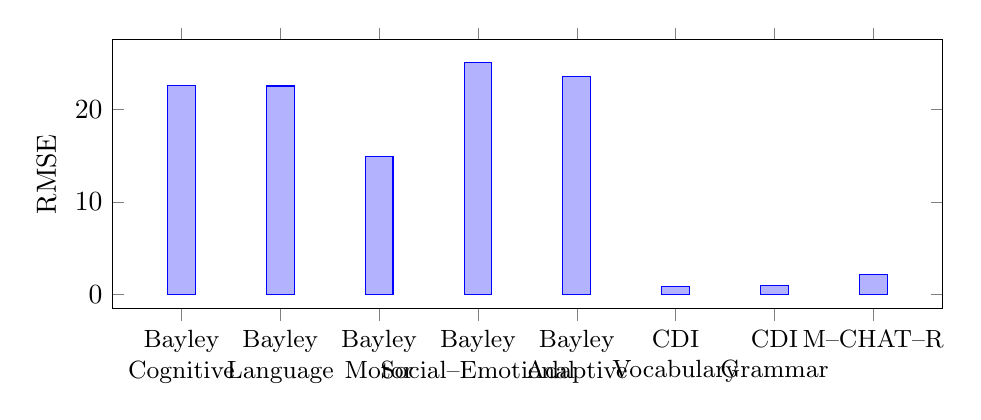
\begin{tikzpicture}
\begin{axis}[
    ybar,
    width=\linewidth, height=5cm,
    ylabel={RMSE},
    symbolic x coords={
        {Bayley\\Cognitive},
        {Bayley\\Language},
        {Bayley\\Motor},
        {Bayley\\Social--Emotional},
        {Bayley\\Adaptive},
        {CDI\\Vocabulary},
        {CDI\\Grammar},
        {M--CHAT--R}
    },
    xtick=data,
    x tick label style={
        align=center,
        font=\small
    },
]
\addplot coordinates {
 ({Bayley\\Cognitive},22.6256) +- (0,3.5908)
 ({Bayley\\Language},22.5436)  +- (0,3.5131)
 ({Bayley\\Motor},14.8806)     +- (0,2.6624)
 ({Bayley\\Social--Emotional},25.1234) +- (0,4.8099)
 ({Bayley\\Adaptive},23.5676)  +- (0,4.8450)
 ({CDI\\Vocabulary},0.8487)    +- (0,0.1777)
 ({CDI\\Grammar},0.9794)       +- (0,0.1457)
 ({M--CHAT--R},2.1652)         +- (0,0.8102)
};
\end{axis}
\end{tikzpicture}

\vspace{0.8cm}

% ---------- R2 ----------
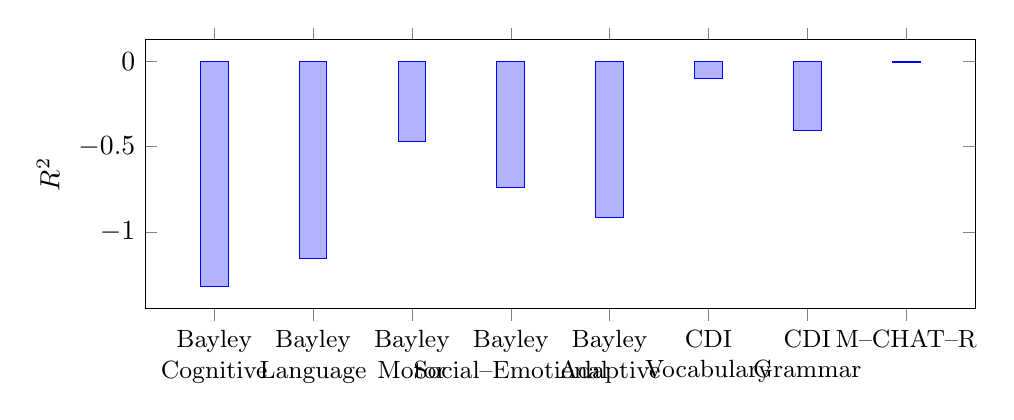
\begin{tikzpicture}
\begin{axis}[
    ybar,
    width=\linewidth, height=5cm,
    ylabel={$R^2$},
    symbolic x coords={
        {Bayley\\Cognitive},
        {Bayley\\Language},
        {Bayley\\Motor},
        {Bayley\\Social--Emotional},
        {Bayley\\Adaptive},
        {CDI\\Vocabulary},
        {CDI\\Grammar},
        {M--CHAT--R}
    },
    xtick=data,
    x tick label style={
        align=center,
        font=\small
    },
]
\addplot coordinates {
 ({Bayley\\Cognitive},-1.3177)
 ({Bayley\\Language},-1.1544)
 ({Bayley\\Motor},-0.4694)
 ({Bayley\\Social--Emotional},-0.7407)
 ({Bayley\\Adaptive},-0.9144)
 ({CDI\\Vocabulary},-0.1021)
 ({CDI\\Grammar},-0.4071)
 ({M--CHAT--R},-0.0065)
};
\end{axis}
\end{tikzpicture}

\caption{XGBoost performance across 8 outcomes (5-fold cross-validation).}
\end{figure}







\end{document}







